\chapter{Experimental Results}
This chapter presents the experimental analysis of the CSMA/CA simulator, comparing the performance of the standard protocol with the adaptive approach based on Reinforcement Learning.

\section{Case Studies}
Here we test two configurations:
\begin{itemize}
    \item \textbf{Standard CSMA/CA:} In this baseline protocol, nodes operate using a Binary Exponential Backoff mechanism. When the medium is sensed busy, a node waits for a \texttt{DIFS} period and then selects a random backoff timer within the range $[0,CW-1]$. The CW starts at a minimum value (\texttt{CW\_MIN}) and doubles after each collision until it reaches a maximum threshold (\texttt{CW\_MAX}).
    \item \textbf{Adaptive CW:} In this model, each node acts as an RL agent that treats the selection of the Contention Window as a Multi-Armed Bandit problem. The node learns to pick the optimal CW size from a set of "arms" based on the rewards received.
\end{itemize}

The motivation behind this choice is to allow nodes to learn the optimal CW size for the current network density. If a node experiences frequent collisions, it will learn to pick larger windows. Instead, if a node receives few transmissions (low traffic in the network), it will learn to pick a smaller window in order to maximize the rewards received over time.

\section{Simulation Parameters}
The simulation parameters, summarized in Table \ref{tab:simulation-parameters}, are configured to reflect a typical WSN scenario.

\begin{table}[]
    \centering
    \begin{tabular}{|>{\raggedright\arraybackslash}                     p{0.20\textwidth}|
                    >{\centering\arraybackslash}p{0.10\textwidth}|
                    >{\raggedright\arraybackslash}p{0.62\textwidth}|}
        \hline
        \textbf{Parameter} &\textbf{Value} & \textbf{Description}
        \\\hline
        \texttt{HORIZON} & $5,000,000$ & The total duration of a single simulation run.
        \\\hline
        \texttt{SIM\_RUNS} & 20 & Number of times the simulation is executed. The results are averaged across these runs.
        \\\hline
        \texttt{SEED} & -1 & Controls the random number generator seed. \texttt{-1} enables a random seed for each simulation run.
        \\\hline
        \makecell[l]{\texttt{DATA\_DUR} \\ \texttt{ACK\_DUR}} & \makecell[c]{4 \\ 1} & The transmission time for data packets and acknowledgments.
        \\\hline
        \makecell[l]{\texttt{SIFS\_DUR} \\ \texttt{DIFS\_DUR}} & \makecell[c]{2 \\ 4} & 
        Short Inter-Frame Space (SIFS) and Distributed Inter-Frame Space (DIFS) durations.
        \\\hline
        \texttt{ACK\_TIMEOUT} & 8 & The maximum time a node waits for an ACK before assuming a collision or loss occurred.
        \\\hline
        \texttt{NODE\_NUM} & 15 & The number of nodes in the network competing for the medium.
        \\\hline
        \texttt{RANGE} & 3 & Transmission range of each node within the monitored area.
        \\\hline
        \texttt{QUEUE\_CAPACITY} & 50 & 
        Maximum number of packets that can be stored in a node’s internal queue. When the queue is full, newly generated packets are dropped.
        \\\hline
        \texttt{GEN\_PROB} & 0.003 & The probability that a node generates a new packet in a given tick.
        \\\hline
        \makecell[l]{\texttt{CW\_MIN} \\ \texttt{CW\_MAX}} & \makecell[c]{15 \\ 1023} & Lower and upper bounds of the contention window used for random backoff.
        \\\hline
        \texttt{SLOT\_TIME} & 1 & The duration of a single backoff slot, which corresponds to the system's atomic tick.
        \\\hline
        \texttt{RL\_EPSILON} & 0.10 & The exploration rate for the $\epsilon$-greedy policy. It defines the probability of choosing a random action.
        \\\hline
        \texttt{RL\_ALPHA} & 0.30 & 
        Controls how fast the learning agent updates its knowledge. It allows the agent to adapt to changing network conditions.
        \\\hline
        \texttt{ARMS\_NUM} & 7 & The number of actions available to the RL agent. Each arm represents a different CW the agent can choose from.
        \\\hline
        \makecell[l]{\texttt{MAREA\_WIDTH} \\ \texttt{MAREA\_HEIGHT}} & \makecell[c]{10 \\ 10} & Define the width and height of the monitored area.
        \\\hline
    \end{tabular}
    \caption{Simulation paramters.}
    \label{tab:simulation-parameters}
\end{table}

To test the policies, we simulate the network under varying conditions:
\begin{itemize}
    \item \textbf{Number of Nodes (\texttt{NODE\_NUM}):} We scale the network from a low-density (5 nodes), medium-density (15 nodes) to a high-density scenario (30 nodes) to observe the impact on collision rates.

    \item \textbf{Packet Generation Probability (\texttt{GEN\_PROB}):} High values simulate a saturated network where nodes almost always have packets to send. We start from sending occasional updates (\texttt{GEN\_PROB} = 0.001), standard load (0.003), to saturated medium where nodes always have packets in the queue (0.005).
    
    \item \textbf{Exploration Rate (\texttt{RL\_EPSILON}):} With low $\epsilon$ (0.01) the node quickly converges to a strategy but may get stuck in a sub-optimal CW if the environment changes. 
    Medium $\epsilon$ (0.10) represents the standard balance between exploration and exploitation.
    With high $\epsilon$ (0.30) the node remains flexible and learns faster in dynamic conditions.
\end{itemize}

\section{Performance Metrics}
To quantify the efficiency of the protocols, we track the following metrics:
\begin{itemize}
    \item \textbf{Packet Delivery Ratio (PDR):} The ratio of successfully acknowledged packets to the total packets generated.

    \item \textbf{Throughput:} The average number of packets successfully received per time unit.

    \item \textbf{Average Latency:} The average time elapsed between the generation of a packet and its successful delivery.

    \item \textbf{Collision Rate:} The ratio of collisions to the total number of transmission attempts.
\end{itemize}

\section{Simulations and Results}
\subsection{Node Density}
The first scenario evaluates how the system scales as the number of nodes increases (5, 10, and 15 nodes). In a high-density environment, the probability of multiple nodes choosing the same backoff slot increases, leading to higher collision rates and lower efficiency.

\begin{table}[ht]
    \centering
    \begin{tabular}{|c|c|c|c|c|c|c|}
    \hline
    \textbf{Nodes} & \textbf{Protocol} & \textbf{PDR} & \textbf{Throughput} & \textbf{Avg Latency} & \textbf{Collision Rate}
    \\\hline
    \multirow{2}{*}{5 (Low)} & Standard & 99.93\% & 0.0314 & 53.65 & 4.57\% \\\cline{2-6}
     & Adaptive & 99.72\% & 0.0200 & 97.43 & 6.72\% \\\hline
    \multirow{2}{*}{10 (Med)} & Standard & 84.57\% & 0.0778 & 386.46 & 14.46\% \\\cline{2-6}
     & Adaptive & 98.65\% & 0.0482 & 182.32 & 10.31\% \\\hline
    \multirow{2}{*}{15 (High)} & Standard & 78.93\% & 0.0916 & 768.10 & 23.46\% \\\cline{2-6}
     & Adaptive & 95.57\% & 0.0722 & 351.27 & 17.77\% \\\hline
    \end{tabular}
    \caption{Experimental results on variable node density.}
    \label{tab:node-density}
\end{table}

The results showed in Table \ref{tab:node-density} clearly show that the Standard CSMA/CA performs slightly better in terms of throughput and collision rate in low-density scenarios. 
This is because the Standard protocol immediately resets the contention window (CW) to $CW_{min}$ after a successful transmission, allowing for faster subsequent access. Adaptive RL, by contrast, maintains a memory of rewards and might "explore" larger CWs or converge to a value larger than $CW_{min}$ to avoid potential collisions, which also adds a small latency penalty.

However, as density increases, the Standard protocol's performance decreases and the Adaptive CW maintains a high PDR and significantly lower latency by learning to avoid collisions through better CW management.
This occurs because the Standard protocol's logic is too aggressive and nodes repeatedly collide at $CW_{min}$ before backing off again. The Adaptive protocol maintains a much higher PDR because the RL agent learns that in high-density environments, a larger CW is the "optimal arm" to minimize collisions.

\begin{figure}[ht]
    \centering
    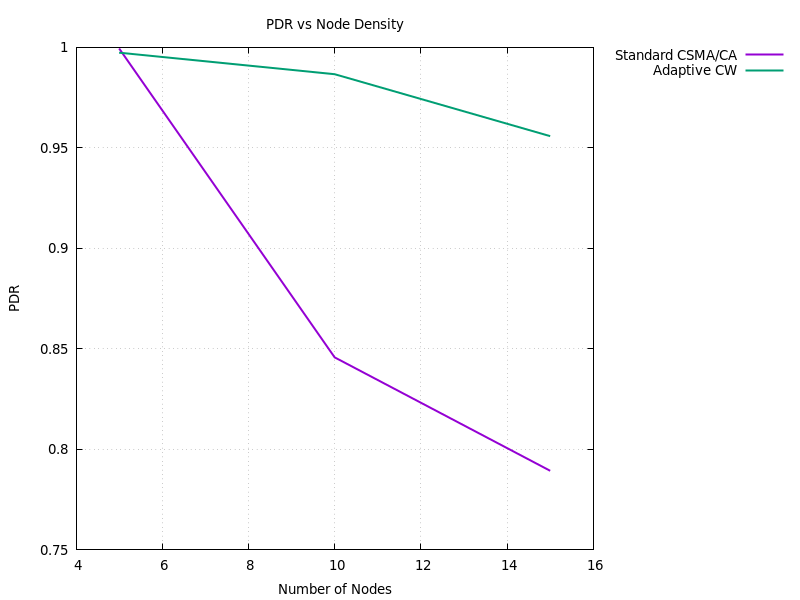
\includegraphics[width=0.8\linewidth]{figures/pdr_vs_density.png}
    \caption{PDR comparison across node densities.}
    \label{fig:node-density-plot}
\end{figure}

This show us how fixed policies are not scalable: the Standard protocol is greedy and fast in low density networks. Instead, the Adaptive approach avoids the congestion by selecting higher contention windows, without waiting for a series of collisions, in higher density networks.

\subsection{Network Traffic}
We also evaluated the system under different traffic loads by varying the packet generation probability.

\begin{table}[ht]
    \centering
    \begin{tabular}{|c|c|c|c|c|c|c|}
    \hline
    \textbf{Gen. Prob.} & \textbf{Protocol} & \textbf{PDR} & \textbf{Throughput} & \textbf{Avg Latency} & \textbf{Collision Rate}
    \\\hline
    \multirow{2}{*}{0.003 (Low)} & Standard & 99.97\% & 0.0491 & 68.65 & 6.52\% \\\cline{2-6}
     & Adaptive & 99.98\% & 0.0294 & 68.33 & 9.13\% \\\hline
    \multirow{2}{*}{0.005 (Med)} & Standard & 95.93\% & 0.0752 & 280.27 & 13.83\% \\\cline{2-6}
     & Adaptive & 98.94\% & 0.0473 & 161.91 & 8.55\% \\\hline
    \multirow{2}{*}{0.010 (High)} & Standard & 70.44\% & 0.0812 & 640.49 & 19.39\% \\\cline{2-6}
     & Adaptive & 78.30\% & 0.0776 & 584.19 & 17.61\% \\\hline
    \end{tabular}
    \caption{Experimental results on variable network traffic.}
    \label{tab:net-traffic}
\end{table}

With low traffic both protocols perform well, with PDR above 99.9\%. In high traffic scenarios both the standard and the adaptive PDRs collapses. 

Here the Adaptive protocol try to balance the latency-throughput trade-off: it prefers to wait longer to ensure a successful delivery rather than attempting frequent transmissions that lead to collisions.

\begin{figure}[ht]
    \centering
    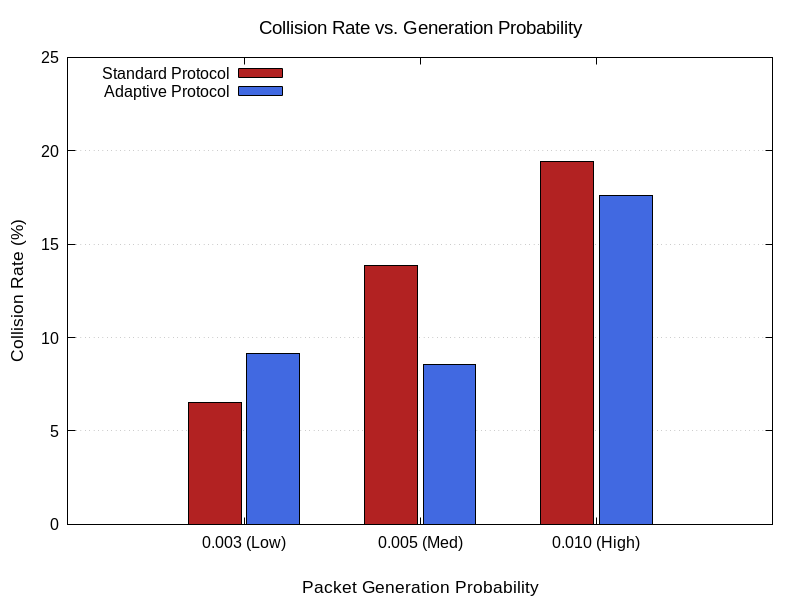
\includegraphics[width=0.8\linewidth]{figures/collision_rate_chart.png}
    \caption{Collision rates under varying traffic.}
    \label{fig:network-traffic-plot}
\end{figure}

\subsection{Learning Rate and Exploration}
Finally, we analyzed the impact of the RL hyperparameters, $\alpha$ (alpha) and $\epsilon$ (epsilon), on the Adaptive CW performance.

\begin{table}[ht]
    \centering
    \begin{tabular}{|c|c|c|c|c|c|c|}
    \hline
    \textbf{$\alpha$} & \textbf{Protocol} & \textbf{PDR} & \textbf{Throughput} & \textbf{Avg Latency} & \textbf{Collision Rate}
    \\\hline
    0.10 & Adaptive & 98.74\% & 0.0470 & 175.41 & 9.63\% \\\hline
    0.20 & Adaptive & 96.43\% & 0.0467 & 267.14 & 10.45\% \\\hline
    0.30 & Adaptive & 94.53\% & 0.0445 & 398.46 & 9.30\% \\\hline
    \end{tabular}
    \caption{Experimental results on variable learning rate.}
    \label{tab:learning-rate}
\end{table}

\begin{table}[ht]
    \centering
    \begin{tabular}{|c|c|c|c|c|c|c|}
    \hline
    \textbf{$\epsilon$} & \textbf{Protocol} & \textbf{PDR} & \textbf{Throughput} & \textbf{Avg Latency} & \textbf{Collision Rate}
    \\\hline
    0.001 & Adaptive & 97.94\% & 0.0486 & 199.37 & 11.03\% \\\hline
    0.010 & Adaptive & 97.97\% & 0.0459 & 209.69 & 9.10\% \\\hline
    0.030 & Adaptive & 98.17\% & 0.0476 & 197.27 & 13.84\% \\\hline
    \end{tabular}
    \caption{Experimental results on variable exploration.}
    \label{tab:exploration}
\end{table}

Testing $\alpha$ values showed that a lower learning rate provided the best PDR. A higher $\alpha$ makes the agent more reactive to changes in network conditions but also increased the probability of instability.
With high $\alpha$ values a single random collision might cause the node to immediately shift its Q-values toward a very large CW, even if the network isn't actually congested, causing unnecessary delays.

Increasing $\epsilon$ showed that moderate exploration is better. The highest PDR and lowest latency were achieved with $\epsilon$=0.030, where the agent frequently checks other CW sizes to adapt to changing network conditions, but at cost of more collisions.

\begin{figure}[ht]
    \centering
    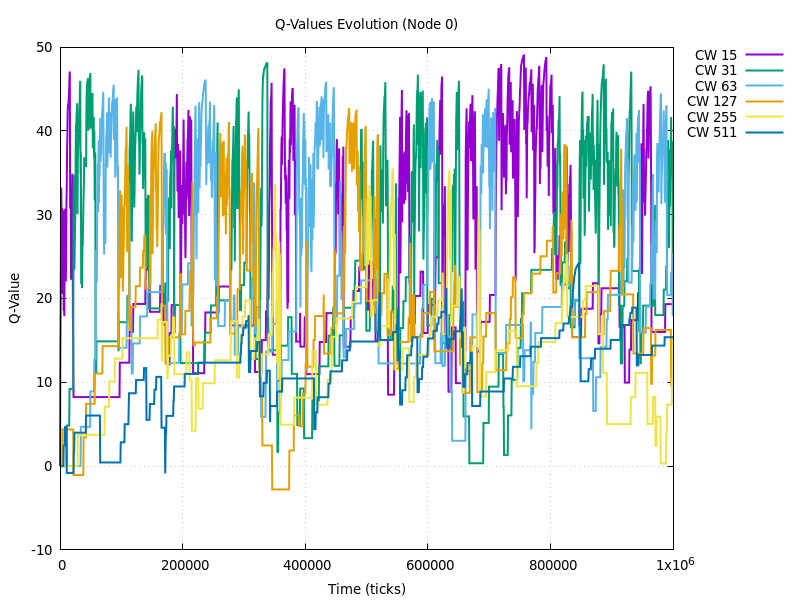
\includegraphics[width=0.8\linewidth]{figures/q_values_over_time.png}
    \caption{Evolution of Q-values over time.}
    \label{fig:q-values-plot}
\end{figure}